\documentclass[review]{elsarticle}
\usepackage{lineno,hyperref, amsmath}
\usepackage{csvsimple}
\usepackage{color}
\usepackage[utf8]{inputenc}
\usepackage{graphicx}

\title{ICBM recalibration}
\author{Lorenzo Menichetti}
\date{January 2021}

\bibliographystyle{elsarticle-num}

%% `Elsevier LaTeX' style
\bibliographystyle{elsarticle-num}

\begin{document}

\begin{frontmatter}

\title{A Bayesian recalibration of the ICBM soil organic carbon model on two sites in northern Europe to include multiple uncertainty sources}

%% Group authors per affiliation:
\author[SLU_ecology]{Lorenzo Menichetti\corref{correspondingauthor}}
\author[SLU_ecology]{Martin Bolinder}
\author[SLU_ecology]{Thomas K{\"a}tterer}


\address[SLU_ecology]{Department of Ecology, Swedish University of Agricultural Sciences (SLU), Uppsala, 75007, Sweden}

\cortext[correspondingauthor]{Corresponding author, lorenzo.menichetti@slu.se}

\begin{abstract}
Abstract here
\end{abstract}

\begin{keyword}
SOC modeling \sep SOC stocks changes \sep ICBM
\end{keyword}

\end{frontmatter}

\linenumbers


%%%%%%%%%%%%%%%%%%%%%%%%%%%%%%%%% SECTION 1
\section{Introduction}
\paragraph{The point} Soil organic carbon (SOC) is the major terrestrial C pool and its management is crucial to the global C budget[1]. The effectiveness of such management relies on the accuracy of our models, not only in terms of simulated predictions but also in quantifying the unavoidable uncertainty associated with them. Uncertainty in SOC models stems from an imperfect knowledge of many components:  i) an error in the measurements itself, ii) the uncertainty in the model structure (for example in the pool definition, even before their interactions), iii) the uncertainty in the edaphic and climatic modules and iv) the uncertainty in the input estimation. All these error components contribute to reduce the robustness of our estimates when it comes to future predictions.
In order to address this problem, it is first of all needed to estimate the uncertainty generated in our model by all these sources of errors in some sort of objective way. This can be done with stochastic calibrations, which can consider the probability distributions of each input variable to the model according to most current estimates and calculate the updated probability distribution of the variables and of predictions after the model is compared with the measurements. There are several possible implementations of this concept; in this study we used formal Bayesian statistics and a classical Metropolis-Hastings sampler. All the possible implementation achieve in any case the similar aim of estimating the error of our predictions and models. An error estimate associated with predictions is crucial to implement environmental policies.
Stochastic calibrations opens up also for a flexible integration of multiple information sources, such as the simultaneous inclusion of the information from multiple sites in the calibration. This additional information can extend the range of validity of models and the robustness of their prediction.

\paragraph{The present study} In the present study we calibrated a first-order compartmental model, ICBM[2], by integrating together in a Bayesian framework all the most recent knowledge about the parameters and the process they represent and two different sites with a similar experimental setup. We also included in the Bayesian framework the calculation of belowground inputs from aboveground biomass and allometric coefficients, starting from prior distributions of various shoot:root factors and a root:exudate coefficient derived from literature review and producing an updated posterior distribution for each of them. We calibrated the model simultaneously against 60 time series coming from different experimental plots from a 62 years old experiment plus other 32 time series from plots from a 22 years old experiment. Both experiments include a long-term bare fallow that represent a great asset to constrain the old organic matter decay kinetics.
The ICBM model is a relatively simple compartmental model but still able to capture most of the observed variability over SOC time scales (<1 year) and its minimalism has the advantage of avoiding unnecessary complications, maintaining it easily manageable and with an easily defined analytical solution. Its model class, first-order compartmental SOC models, is to date by far the most used approach for global and field scale SOC modelling. The introduction of a detailed error estimation in these models is a way to extend their validity and applicability, and the systematic quantification of the error can contribute to reduce the variability nowadays recorded in earth system models concerning SOC predictions.

\paragraph{Main aims} 
\begin{itemize}
\item Update the ICBM model with roughly 20 years of data, more treatments and one additional site compared to the original calibration from 1997 \cite{Andren1997}
\item Update the structure ICBM model with separate inlet pools for amendments, roots and shoots, which are known to produce different amount of humified material \cite{Katterer2011}
\item Provide a simultaneous multi-objective parameterization, more objective compared to the sequential parameterization in the original calibration from 1997 \cite{Andren1997}
\item Re-calibrate the ICBM model within a Bayesian framework to provide a detailed uncertainty estimates of the predictions
\item Estimate the uncertainty of the ICBM model with special focus on the belowground biomass calculation
\item Provide a comprehensive and consistent software package for the estimation of the climatic module
\item Testing the calibrated model over a wide range of soil conditions and climates to assess its boundaries
\end{itemize}
%%%%%%%%%%%%%%%%%%%%%%%%%%%%%%%%% SECTION 2
\section{Material and methods}

%%%%%%%%%%%%%%% SUBSECTION (Data)
\subsection{The data}

%%% SUBSUBSECTION (Experiment)
\subsubsection{The field experiments}
The present study is mainly based on data from the Ultuna Long-Term Frame Experiment, initiated in 1956 in Ultuna (Sweden) and on which the original ICBM calibration was based \cite{Andren1997}, and on a sister experiment initiated in 1996 in Lanna (Sweden) \cite{Katterer2014}.
The Ultuna site is located on a \textit{Typic Euthrochrept} close to Uppsala (59.82$^{\circ}$N, 17.65$^{\circ}$E) and presents 15 treatments (Table  \ref{table:sites}). The site has been cultivated for centuries since before the start of the experiment \cite{Katterer2011}, and since the stard many different crops have been grown on it (cereals, root crops, oil crops, and in the last 17 years silage maize). The annual mean total precipitation is 542 mm and annual mean temperature 5.8$^{\circ}$ C. The plots are relatively small, measuring 2$\times$2 m, and are separated by metal frames extending about 30cm below the soil surface and 10 cm above\\

The site in Lanna (58.34$^{\circ}$N, 13.10$^{\circ}$E) is established on a \textit{Aquic Haplocryept}, and presents only 9 treatments (Table  \ref{table:sites}).
At Lanna only cereals (Oats and Barley) were grown since the beginning of the experiment. The annual mean total precipitation is 636 mm and annual mean temperature 7.3 $^{\circ}$ C. Plots are much bigger size than in Ultuna, measuring between 112 and 92 m$^2$ \\
Both experiments present a randomized block design with four blocks and receive biannual applications of organic matter in known amount of C (roughly 4 Mg ha$^{-1}$ in Lanna\cite{Katterer2014} and roughly 3 Mg ha$^{-1}$ in Ultuna\cite{Katterer2011}), and after harves the biomass is removed. Both experiments present a long term bare fallow (LTBF) treatment, which since the start of each experiment is kept free from vegetation. In Ultuna weeds are removed manually, while in Lanna, due to the size of the plots, with three mechanical treatments per year. This causes more interferences from weeds that sometimes manage to grow in the Lanna LTBF, while Ultuna (due also to its extrme proximity to the SLU Campus and consequent stricter management) is virtually devoid of vegetation. All plots are ploughed in the autumn after harvest.\\
Every year (and more irregularly a few decades ago) soil is sampled after harvest and stored in a soil bank for future analyses. Soil C \% is also measured 


%%% SUBSUBSECTION (SOC)
\subsubsection{SOC measurements and equivalent soil mass calculation}
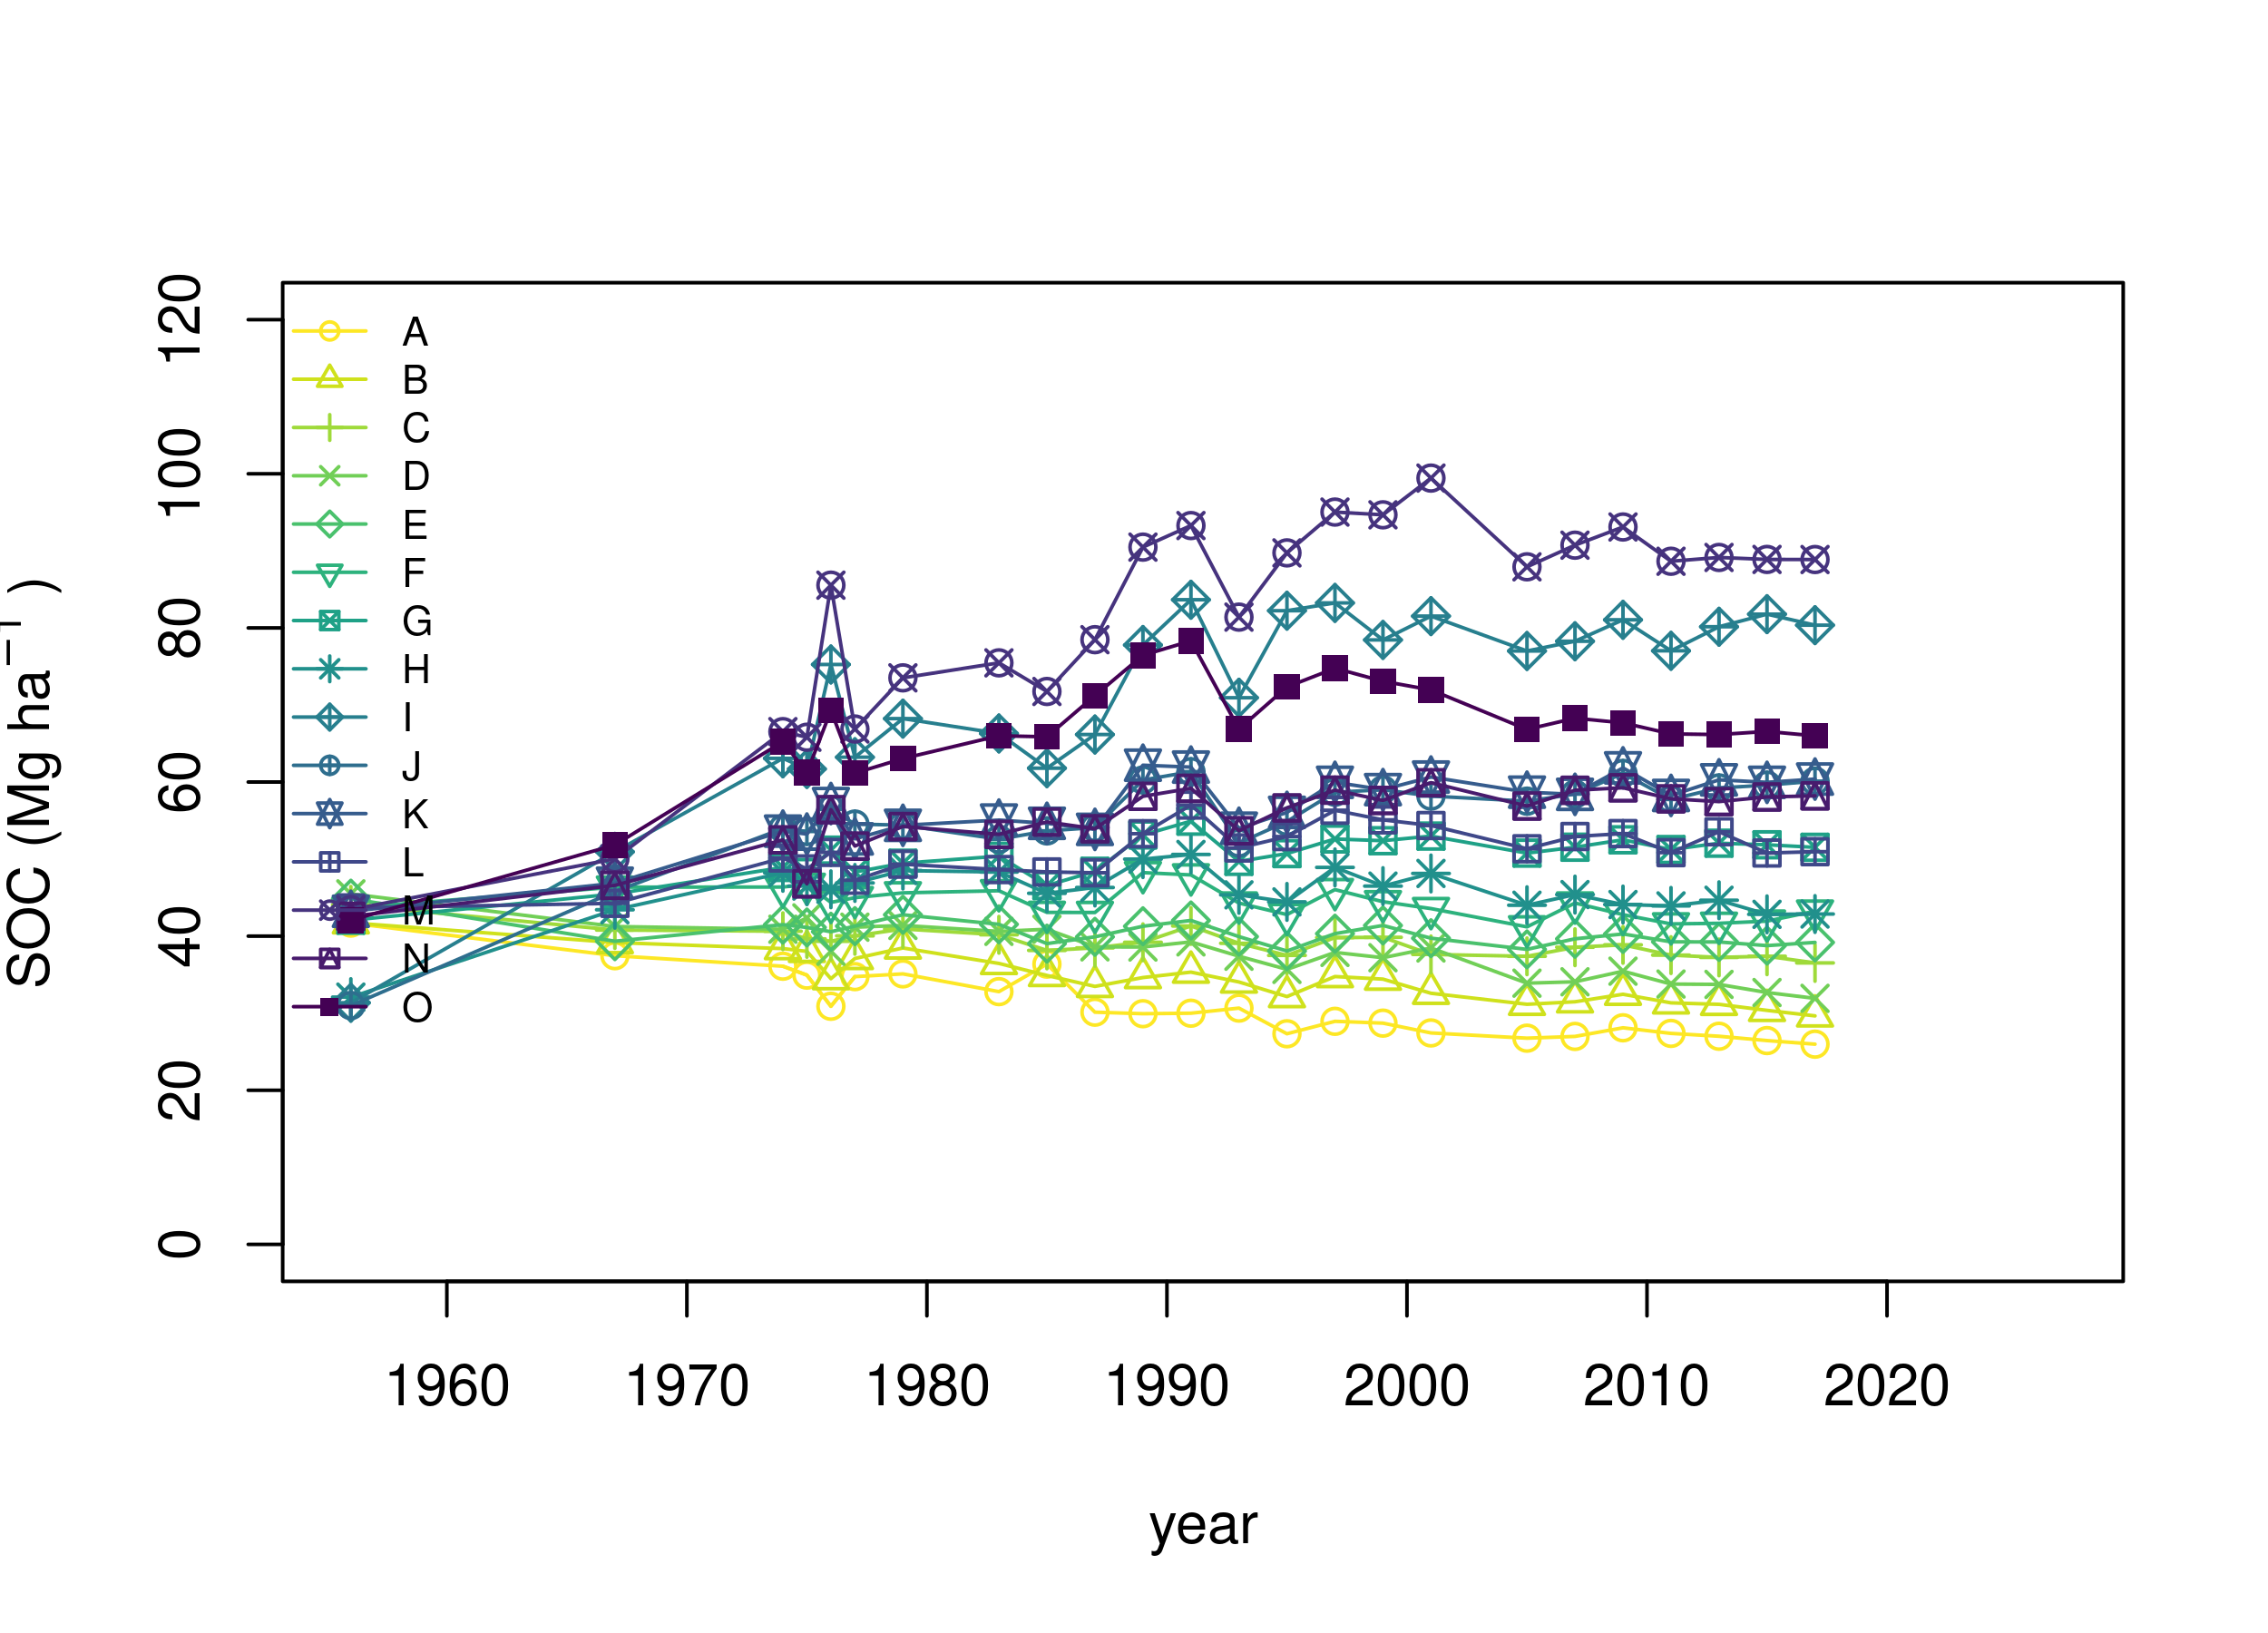
\includegraphics[width=\textwidth]{Ultuna_SOC_data_used.png}

In particular in the older site of Ultuna differences in surface elevation between the plots, due to the mineral removed with sampling over the years but most of all to the different C balance in the different treatments (and also consequent different bulk density). This makes the reference depth of 20 cm shift over time, introducing an erroir that must be compensated for. We corrected in both experiments for the shift of the 20 cm layer according to \cite{Katterer2011}.


%%% SUBSUBSECTION (Biomass)
\subsubsection{Biomass measurements}





%%%%%%%%%%%%%%% SUBSECTION (Model)
\subsection{The model}
The SOC decay model we calibrated is derived from the original ICBM model \cite{Andren1997} with very few modifications.
The original model \cite{Andren1997} considered two decaying pools, "young" (Y) and "old" (O), connected by a humification function. The Y pool represents the organic matter not yet humified, comparable to litter, and decays with really fast kinetics (around 1.25 years of mean residence time), while the O pool represents the organic matter that becomes protected in the soil and decays with much slower kinetics  (around 165 years of mean residence time).\\
This is in general enough to represent observed SOC data \cite{Andren2004}, but more recent studies pointed out the different characteristic of different substrates in terms of humification \cite{Katterer2011}. In order to consider different materials, and their different humification coefficients (which represent the amount of such material that gets humified, or passes to the slower pool), we introduced three separate Y pools, all decaying in parallel. This does not modify the fundamental kinetic of the model neither complicates much the model solution, which can still be found analytically, but allows us to consider the new available information on the decay of the different materials\cite{Katterer2011} into the model calibration (Figure \ref{figure:ICBM_schema}).\\
The mathematics of the ICBM model has been extensively and clearly introduced before in the literature and we refer the reader to former publications for the relative equations (in particular \cite{Katterer2011} and \cite{Katterer2001}).



%%%%%%%%%%%%%%% SUBSECTION (Forcing variables)
\subsection{The model climatic functions}
The ICBM model is relatively simple and therefore quite modular. Its structure allows for easily introducing kinetic modifiers.
Climatic interactions with decomposition are considered as a multiplier of the two decay kinetics $k_y$ and $k_o$. This term is conventionally called $re_{crop}$, and it summarizes all the external influences on decomposition. The term $re_{crop}$ is normalized by convention assuming it as 1 in the Ultuna site, chosen as reference since the model was originaly developed on this site. The $re_{crop}$ calculated from the forcing variables (such as the climatic data) is then rescaled accordingly. The $re_{crop}$ value is calculated based on daily data, but is then averaged annually (since the ICBM model works in annual time steps).\\
This structure allows the ICBM model to be extremely modular, and the term $re_{crop}$ can be modified easily. Over the years its calculation has been updated a few times \cite{Andren2004}, but the term considers always the effect of soil temperature and relative soil moisture (expressed as fraction of active soil water, betweel field capacity and wilting point) on the decay kinetics.\\
The effect of soil temperature is the easiest to calculate, and it is based on a quadratic response function \cite{Andren2004} with maximum ($T_{max}$) set to 30$^{\circ}$ C and minimum ($T_{min}$) set to -3.8$^{\circ}$ C. 
\begin{equation}
re_{temp, t}=\frac{(T_{soil, t}-T_{min})^2}{(T_{max}-T_{min})^2}
\label{equation:retemp}
\end{equation}

This functions presents a curve that is quite similar in shape to the more conventional Arrhenius function \cite{Lloyd1994} and it is pretty well tested. Its limits of applicability are represented by the lack of a protein denaturation mechanism, which varies depending on different soils but happens at relatively high temperature ($>$35$^{\circ}$ C \cite{Ratkowsky2005}) which are in general not reached in soils (and if they are, they persist for relatively short time span and have therefore a minimal influence on the annual average). The daily mean soil temperature is calculated from daily mean temperature based on an empirical relationship:
\begin{equation}
T_{soil, t}=max(-2, 0.92T_{air, t})
\label{equation:soiltemp}
\end{equation}\\

The effect of soil water content is more complicated to simulate, since it is seldom available and in general it must be calculated from many meteorological data. The response function for soil moisture is adapted from \cite{Moyano2013}: 
\begin{equation*}
re_{wat,t} = \begin{cases}
0
&\theta_t< \theta_m\\

\frac{\theta_t-\theta_{th}}{min(\theta_{opt},\theta_{fc})-\theta_{th}} 
&\theta_{th} \leq \theta_t < min(\theta_{opt},\theta_{fc}) \\

1 & min(\theta_{opt},\theta_{fc}) \leq \theta_t \leq \max(\theta_{opt},\theta_{fc})\\

1-(1-r_s)\frac{\theta_t-max(\theta_{opt},\theta_{fc})}{\theta_s-max(\theta_{opt},\theta_{fc})} &  -max(\theta_{opt},\theta_{fc})< \theta_t \leq \theta_s

\end{cases}
\label{equation:rewat}
\end{equation*}
where $\theta_{opt}$, the optimal water content for decomposition, is calculated according to $\theta_{opt}=0.2+1-26 \cdot \theta_{fc}^{2.03}$ and $\theta_{th}$, the lower boundary water content for decomposition, is calculated according to $\theta{th}=0.0965 \cdot \ln{\theta_{wp}}+0.3$, $\theta_{fc}$ is the water content at field capacity, $\theta_{wp}$ is the water content at wilting point, and $r_s=0.5$. But this function needs as input, besides soil hydrological constants, the soil water content. This is seldom available, but can be calculated based on a simulated daily soil water balance once precipitation and evapotranspiration are known. For a certain soil layer of a given thickness the water balance at a given time ($\Omega_t$) can be calculated according to:
\begin{equation}
\Omega_t= \Omega_{t-1}+PPT_t-ET_t-P_{intercepted, t}-\Omega_{bypass, t}
\label{equation:waterbal}
\end{equation}
where $PPT_t$ is the total precipitation in a give day $t$, $ET_t$ is the actual evapotranspiration on the same day, $P_{intercepted, t}$ is the water intercepted by the crop and $\Omega_{bypass, t}$ is the excess water (lost by percolation). 

The $ET_t$ is calculated from reference evapotranspiration ($ET_0$) through two coefficients according to $ET_t=ET_0 \cdot K_c \cdot K_r$, where $K_c$ is the coefficient to calculate the potential evapotranspiration on the specific plot from the reference ($ET_c=ET_0 \cdot K_c$). The factor $K_c$ is calculated from the green area index ($GAI$)according to $K_c=1.3-0.5\cdot e^{-0.17\cdot GAI}$
The intercepted water $P_{intercepted, t}$ is calculated according to the GAI according to $P_{intercepted, t}=min(PPT_t, ETc, GAI\cdot0.2)$.
The factor $K_r$ is a coefficient to consider the effect of water stress on the crop, and it is calculated according to $K_r=max\left(0,\left(1-\frac{0.9\cdot \theta_{fc}-\theta_{t}}{0.9\cdot tfield-0.7\cdot \theta_{wp}}\right)^2\right)$.
Wilting point ($\theta_{wp}$) and field capacity $\theta_{fc}$) are calculated according to pedotransfer functions developed for Sweden by \cite{Katterer2006}.\\
The two climatic scaling factors $re_{temp}$ and $re_{wat}$ are utilized to calculate the interaction bewteen them $re_{x}=re_{temp}\cdot re_{wat}$, which is then rescaled to Ultuna according to the original rescaling factor of 0.10516 \cite{Andren1997}. We decided to mantain the original scaling factor instead of updating it with the new calculation (which is slightly different) for keeping more compatibility with the literature, since the rescaling is anyway an arbitrary standardization.\\
The set of functions for calculating the climate scaling factors has been compiled into an experimental R package, available on the GitHub repository of the corresponding author, available through the package \texttt{devtools} with the following code:
\begin{lstlisting}[language=R]
# load the libraries needed to install from GitHub
library(devtools)
# install the package from the author's GitHub repository
# forcing reinstallation to keep the package up to date
install_github("ilmenichetti/reclim", force=T) 
\end{lstlisting}
Please contact the corresponding author (and maintainer of the package) to report possible bugs, errors or to discuss or suggest changes. 

\begin{figure}[bt]
\centering
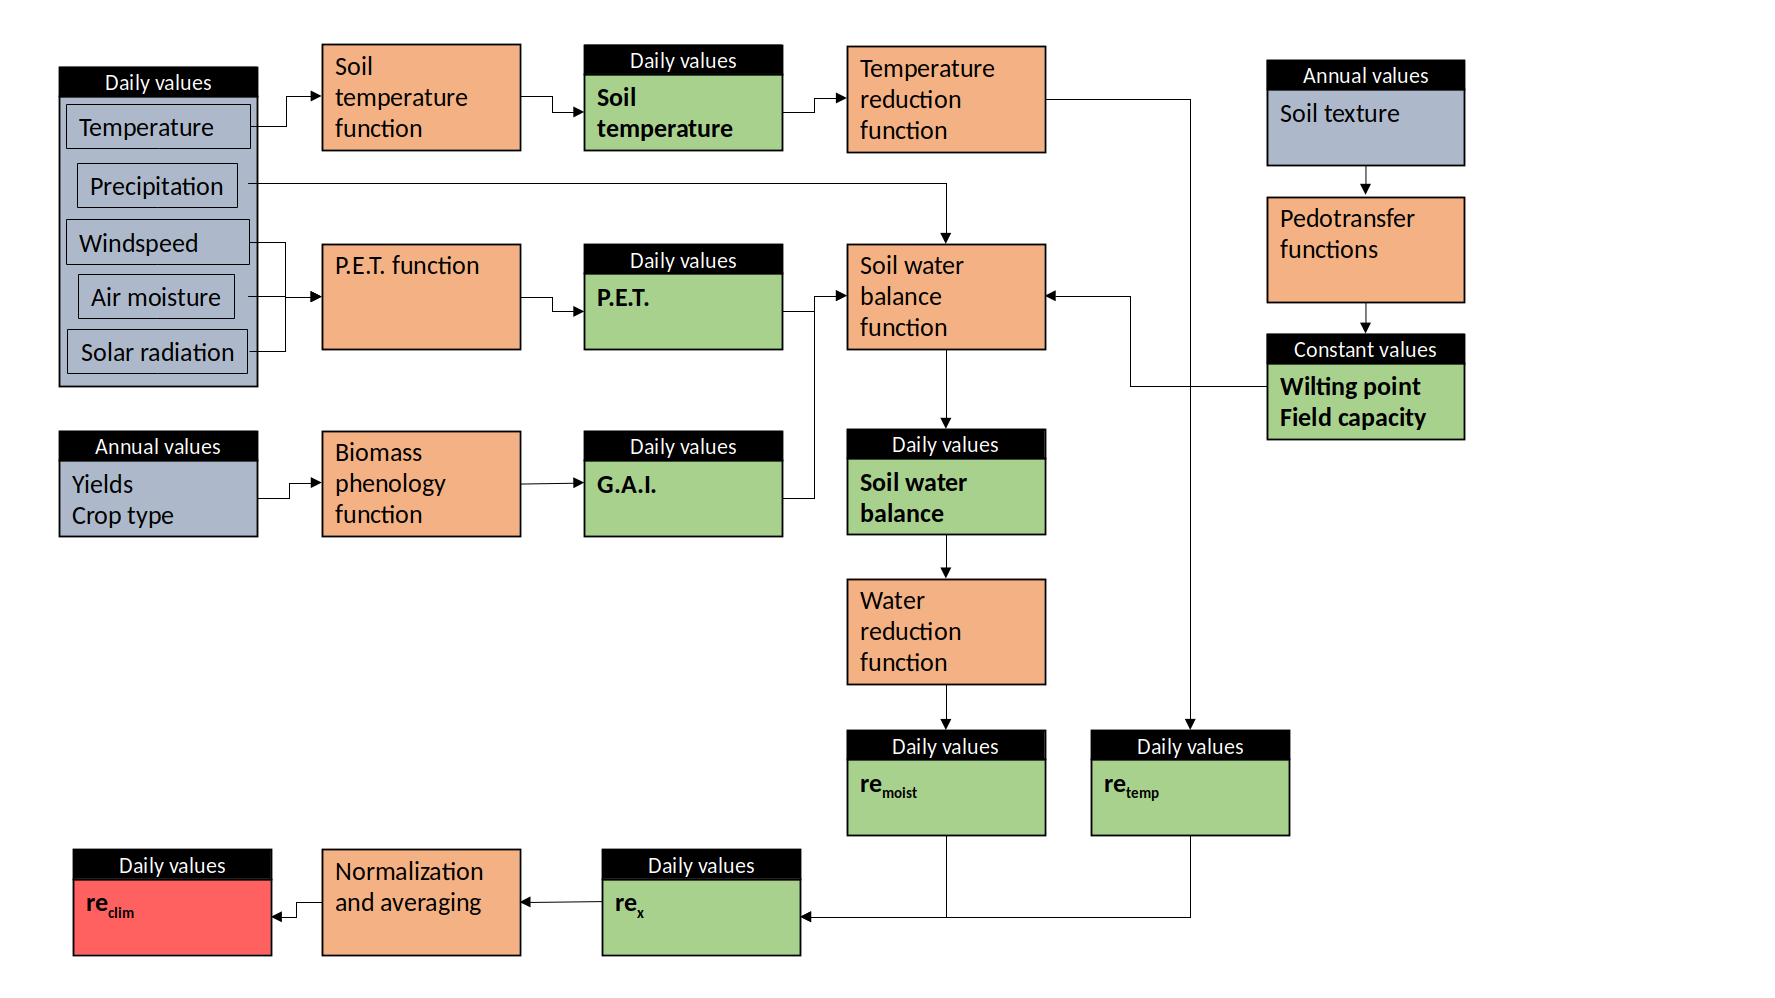
\includegraphics[width=\textwidth]{./Manuscript_plots/re_Clim_schema_reduced.png}
\caption{A schema of the information flow in the climatic module}
\label{figure:reclim}
\end{figure}


%%%%%%%%%%%%%%% SUBSECTION (Calib)
\subsection{Model calibration and initialization}
The decomposition model ha been calibrated within a Bayesian framework, writing the model in JAGS language \cite{JAGS} and running it in R \cite{R-Development-Core-Team2019}. The techniques is nowadays broadly adopted and we refer the reader to more specific publications for details, for example \cite{Kruschke2013, JAGS, AndrewGelman2004}.\\
The climatic scaling has been kept outside the Bayesian framework, and has been calculated (according to the functions described above) for each site and utilized as external driving variable.

The priors for what concerns the model parameters have been selected based on former model calibrations. Each parameter was defined by a truncated Gaussian distribution centered in the former value from the literature, with coefficient of variation 0.15 and  within boundaries between $-0.1\cdot parameter$ and $+0.1\cdot parameter$.\\

As every compartmental SOC model, ICBM needs to be initialized. This means to define the initial C mass in each compartment of the model at time 0. In this study we treated the initial proportion between the $O$ and the sum of all the $Y$ pools as an unknown parameter. The prior was assumed as a truncated Gaussian distribution, centered in 0.93 and with coefficient of variation of 0.1, for both Ultuna and Lanna. The distribution was truncated between 0.9 and 0.95.

\subsubsection{The belowground biomass calculation}
The priors for the shoot to root values have been centered according to \textcolor{red}{Martin references or description here}, with S:R=11 for cereals, S:R=30 for root crops, S:R=8 for oil seeds and S:R=6.25 for corn. Since the uncertainty of the belowground estimation was one of the focuses of the study we assumed less strong priors than for the model parameters. The coefficient of variation has been assumed as 0.25 for all the ratios, and the distributions were not truncated.

\subsubsection{Dealing with a few unknowns}
The experiments present some potentially unknown errors that were treated statistically adding uncertain priors. In both sites all the aboveground biomass is removed, but some organic material is left in the field as stubbles. In Ultuna we assumed a value of 4$\pm$1\% of the total aboveground biomass, while in Lanna some measurements were available \textcolor{red}{references or description here. From where do these data come from?} and we assumed 17$\pm$5\%. Please consider that the Ultuna site is managed by hand and therefore with much more precision than in Lanna and the assumed error is already relatively large.\\
Another possible problem is the contaminations of the bare fallow treatments. Here we would assume no inputs because of the continuous removal of vegetation, but some plant might sometimes grow unnoticed.
The Ultuna treatment is really close to the campus of the institution of the authors, and it is checked with almost daily frequence. Contaminations are here extremely low and in general no weed ever manage to grow, but there might be in some seasons a biofilm that can include some photosinthetic algae.
The Lanna treatment is of more difficult management, being located relatively far from the mother institution and in particular because of the much larger extension of the plot, which makes impossible a manual weeding. The bare fallow treatment in Lanna is kept free from vegetation through three susequent disc harrowing during each growing season, and this leads to much more contaminations in Lanna in particularly favourable seasons.
We dealt with this uncertainty adding an error term in the input estimation for the LTBF (which is assumed zero). This term was assumed with an uniform distribution between 0 and 5\% of the aboveground biomass recorded in the control treatment in Ultuna, and 50\% of the aboveground biomass recorded in the control treatment in Lanna.


%%%%%%%%%%%%%%%%%%%%%%%%%%%%%%%%% SECTION 3
\section{Results}

%%%%%%%%%%%%%%%%%%%%%%%%%%%%%%%%% SECTION 4
\section{Discussion}

%%%%%%%%%%%%%%%%%%%%%%%%%%%%%%%%% SECTION 5
\section{Conclusions}

\end{document}
